%\newpage
%\subsection{Dataset}

Next, we apply our method to brain imaging data from the anonymized multimodal
neuroimaging ``Mother Of all Unification Studies'' (MOUS) dataset
\citep{schoffelen2019204}. The dataset contains magneto-encephalography (MEG)
recordings of 102 healthy native-Dutch adults who participated in a reading
task. Twelve subjects were excluded from the analysis because of corrupted file headers.
%
Subjects were exposed to a rapid serial visual presentation of Dutch words. The
word lists consisted of 120 sentences, and scrambled lists of the same words.
Each word was presented on the computer screen for 351ms on average (min: 300ms,
max: 1400ms). Successive words were separated by a blank screen for 300ms, and
successive sentences were separated by an empty screen for a few (3-4) seconds.

\subsubsection{MEG preprocessing}

The raw MEG data was bandpass-filtered between 0.1 and 40Hz using MNE-Python
default parameters \citep{gramfort2013meg, gramfort2014mne}. Specifically, we used a zero-phase finite impulse
response filter (FIR) with a Hamming window and with transition bands of 0.1Hz
and 10Hz for the low and high cut-off frequencies. The raw data was then segmented 100ms before word onset and 1s after
word onset ($t=0$ms corresponds to word onset). Finally, each resulting
segment was baseline-corrected between -100ms and 0ms, and decimated by 5 and
thus led a sampling frequency of 240Hz. The average responses across words is displayed in \ref{fig:meg_evoked}
For each subject and each time sample relative to word onset, we
build an observation matrix $Y \in \mathbb{R}^{n \times d_y}$ of $n\approx$ 2700 words
by $d_y=301$ MEG channels (273 magnetometers and 28 compensation channels). Each
of the columns of $Y$ is normalized to have zero mean and unit variance.


\begin{figure}[t!]
  \centering
  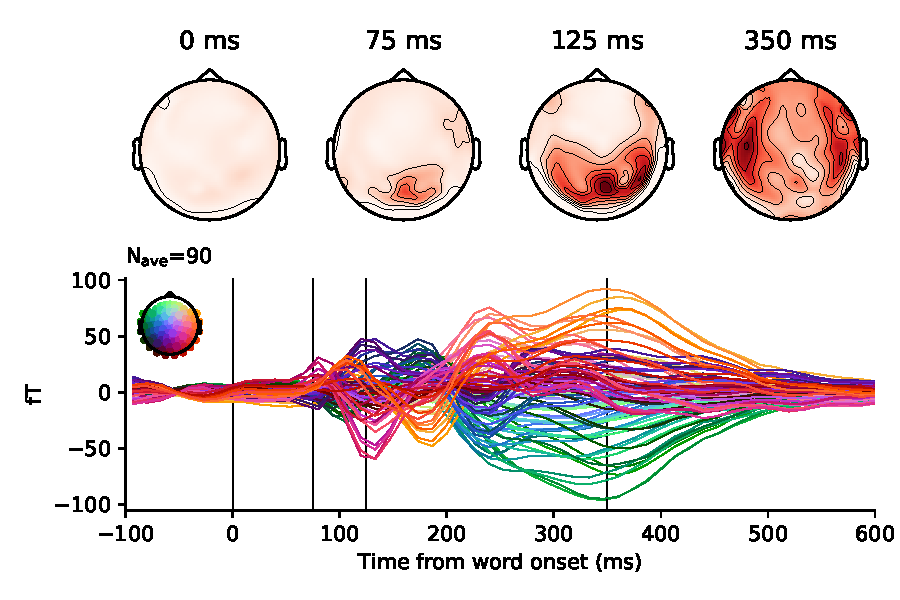
\includegraphics[width=\textwidth, trim=0cm 0cm 0cm 0cm, clip=True]{figures/meg_evoked.pdf}
  \caption{102 subjects read $\approx$ 2,700 words while their brain activity was recorded with MEG. Top. Average brain response to words relative to their onset (gradiometers), as viewed from above the head. Bottom. Each line represents a MEG sensor (magnetometer), color-coded by spatial position. Posterior responses, typical of primary visual cortex activity, peak around 100 ms after word onset and are followed by an anterior propagation of activity typical of semantic processing in the associative cortices. Vertical lines indicate moments of above topographies.
  }
  \label{fig:meg_evoked}
\end{figure}

\subsubsection{Feature definition}

When human subjects read words, the number of letters is known to modulate
brain activity from 100ms after word onset \citep{pegado2014timing}.
Similarly, word frequency is known to modulate brain activity around 400ms
\citep{kutas2011thirty}. In the present study, we consider these two well-known features, as well as an untested feature ('Word Function') and dummy variable.
%
"Word Length' refers to the total number of letters, and is expected to specifically cause a variation in the early evoked MEG responses (i.e. from 100 ms after stimulus onset) elicited by the retinotopically-tuned visual cortices.
%
'Word Frequency', as derived with WordFreq \citep{speerwordfreq}, indexes how frequently each word appears in Dutch (using the Zipf logarithmic scale of \citep{van2014subtlex}). This feature is expected to specifically cause a variation in the late evoked MEG responses (i.e. from 400 ms), because it variably engages semantic processes in the temporal cortices \citep{kutas2011thirty}.
%
Finally, 'Word Function' indicates whether each word is a content word (i.e. a noun, a verb, an adjective or an adverb) or a function word (i.e. a preposition, a conjunction, a determinant, a pronoun or a numeral), and was derived from Spacy's part of speech tagger \citep{spacy2}. To our knowledge, this feature has not been thouroughly investigated with MEG. Its causal contribution to reading processes in the brain is thus largely unknown.
%
To verify that B2B and other models would not inadequately identify non-causal features, we added a dummy feature, constructed from a noisy combination of "Word Length" and "Word Frequency":
\begin{equation}
  dummy = z(length) + z(frequency) + \mathcal{N}
\end{equation}
where $z$ transforms features into zero-mean and unit variance vectors and $\mathcal{N}$ is random vectors sampling a zero-mean unit-variance Gaussian distribution.

This procedure yields an $X \in \mathbb{R}^{n \times d_x}$ matrix of $n\approx$ 2700 words by
$d_x=4$ features for each subject. Each of the columns of $X$ is normalized to
have a mean and a standard deviation of 0 and 1 respectively.

\subsubsection{Models and statistics}

We compare B2B to four standard models: forward regression, backward regression, CCA and PLS, as implemented in scikit-learn, and optimized with nested cross validation over twenty l2 regularization parameters logarithmically spaced between $10^-4$ and $10^4$ or 1 to 4 caconical components.

We used the feature importance described in \ref{algorithm:b2b_fi} to assess the extent to which each feature $X_i$ specifically improves the prediction of held-out $Y$ data.

Each model was implemented for each subject and each time sample independently. Pairwise comparison across models were performed using a wilcoxon test on the $\Delta R$ averaged across time.

Corresponding results can be found in Figure \ref{fig:meg_results}. Significant pairwise differences across models are highlighted with the top horizontal bars in \ref{fig:meg_results}.

\begin{figure}[t!]
  \centering
  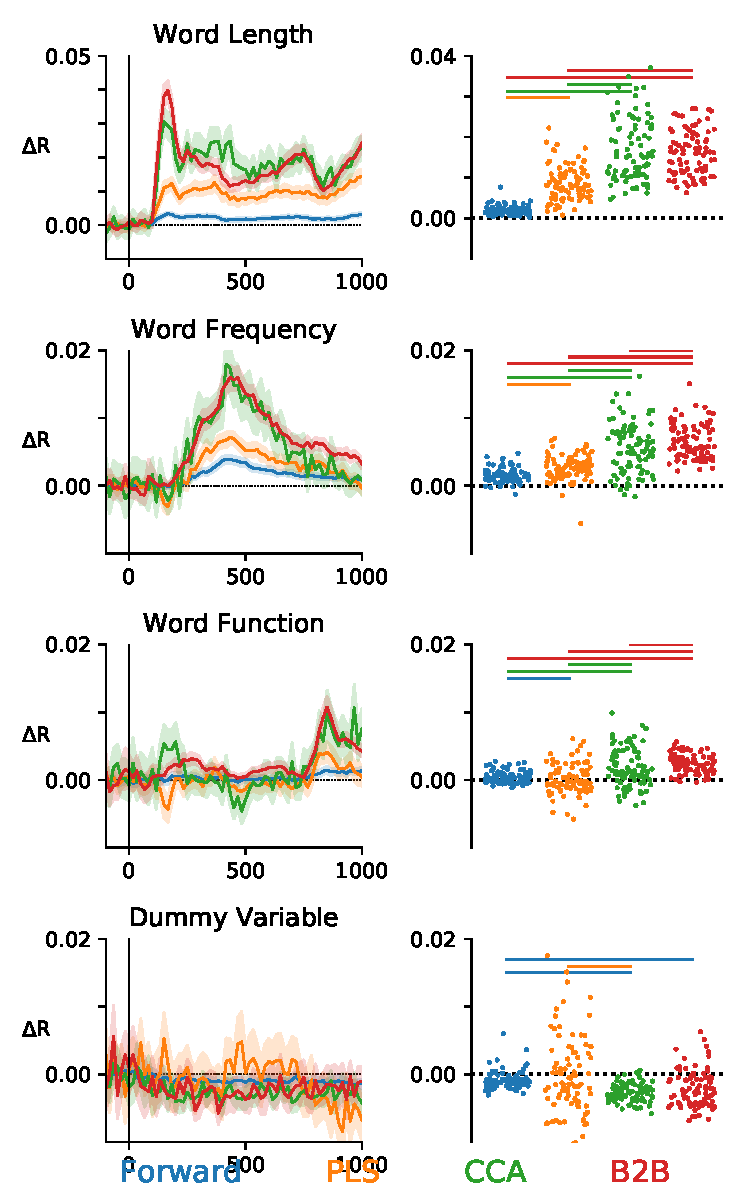
\includegraphics[width=\textwidth, trim=0cm 0cm 0cm 0cm, clip=True]{figures/meg.pdf}
  \caption{Forward regression (Blue), PLS (orange), CCA (green) and B2B (red) are compared on their ability to reliably predict single-trial MEG signals evoked by words. Left. Average improvement of correlation coefficient $\Delta R$ obtained on held-out data when each of the four features "Word Length", "Word Frequency", "Word Function" and "Dummy Variable" was provided to the model \ref{algorithm:b2b_fi}. Error bars indicate standard error of the mean (SEM) across subjects. Right. Average $\Delta R$ across time. Each dot represents a subject. The top horizontal lines indicate significant differences between pairwise comparison across models, color coded by the winning model. B2B outperforms all models on meaningful features, at the exception of CCA for the "word length".}
  \label{fig:meg_results}
\end{figure}

\subsubsection{Results}
We compared the ability of Forward regression, Backward regression, CCA, PLS and B2B to estimate the causal contribution of four distinct but collinear features on brain evoked responses to words.

First, \ref{fig:meg_supp} shows that the Backward model decodes the dummy variable well above chance level. In addition, "Word Length" and  "Word Frequency" present a similar decoding time course, even though these features are known to influence early and late MEG responses respectively \citep{kutas2011thirty}. These results illustrate the well-known fact that backward modelling cannot be used to estimate the causal contribution of collinear features.

We thus focus on valid modeling (Forward Regression, PLS, CCA, and B2B) and estimate the change of correlation coefficients $\Delta R$ induced by the introduction of each feature into the model \ref{algorithm:b2b_fi}. As expected, none of the models significantly predicted the 'Dummy Variable' to be a causal factors (i.e. $\Delta R < 0$ for all models, all $p > .089$)


Figure \ref{fig:meg_results} shows, for each model, the effects obtained across time (left) and subjects (right).


The results show that all models significantly detect that both word length and
word frequency modulate brain responses after word onset. However,
forward regression detected word length ($t$-value$=10.6$, $p=10^{-16}$) and
word frequency ($t$-value$=11.1$, $p=10^-17$) less reliably than B2B (length:
$t$-value$=18.7$, $p=10^{-31}$, frequency: $t$-value$=15.9$, $p=10^{-26}$). B2B
was less sensitive than the backward regression (length: $t$-value$=33.6$,
$p=10^{-50}$, frequency: $t$-value$=31.7$, $p=10^{-48}$). However, as backward models confound collinear factors, this high sensitivity likely comes from a loss of specificity. This possibility is corroborated by the fact that the effects of word length and word frequency identified with backward regression present largely similar dynamics.

Finally we investigate in Figure \ref{fig:megresult} whether B2B was sufficiently sensitive to reliably detect a multiplicity of subtle features, such as individual letters and part-of-speech. The vast majority of the visual and lexical features appeared to be reliably detected (see Figure 4 in Supplementary Material). B2B thus promises to improve the detectability of subtle effects.
